\setcounter{section}{8}
\setcounter{subsection}{0}

\section{Estudo da Variação das Funções}

% ==============================================================================
% 9.1. TEOREMA DO VALOR MÉDIO (TVM)
% ==============================================================================
\subsection{Teorema do Valor Médio (TVM)}
\textit{Esta subseção não possui exercícios.}

\clearpage

% ==============================================================================
% 9.2. INTERVALOS DE CRESCIMENTO E DE DECRESCIMENTO
% ==============================================================================
\subsection{Intervalos de Crescimento e de Decrescimento}

\begin{exercicio}[1]
Determine os intervalos de crescimento e de decrescimento e esboce o gráfico (calcule para isto todos os limites necessários):
\begin{enumerate}[label=\alph*)]
    \item $f(x) = x^3 - 3x^2 + 1$
    \item $f(x) = x^3 + 2x^2 + x + 1$
    \item $f(x) = x + \dfrac{1}{x}$
    \item $y = x^2 + \dfrac{1}{x}$
    \item $y = x + \dfrac{1}{x^2}$
    \item $f(x) = 3x^5 - 5x^3$
    \item $x = \dfrac{t}{1 + t^2}$
    \item $x = \dfrac{t^2}{1 + t^2}$
    \item $x = 2 - e^{-t}$
    \item $y = e^{-x^2}$
    \item $f(x) = e^{2x} - e^x$
    \item $g(t) = e^{\frac{1}{t}}$
    \item $f(x) = \dfrac{x^3 - x^2 + 1}{x}$
    \item $f(x) = \dfrac{3x^2 + 4x}{1 + x^2}$
    \item $g(x) = x e^x$
    \item $f(x) = -x^4 + 4x^3 - 4x^2 + 2$
    \item $f(x) = \dfrac{e^x}{x}$
    \item $g(x) = \dfrac{x^2 - x + 1}{2(x - 1)}$
    \item $f(x) = \dfrac{\ln x}{x}$
    \item $g(x) = x - e^x$
\end{enumerate}
\end{exercicio}

\begin{exercicio}[2]
Prove que a equação $x^3 - 3x^2 + 6 = 0$ admite uma única raiz real. Determine um intervalo de amplitude 1 que contenha tal raiz.
\end{exercicio}

\begin{exercicio}[3]
Prove que a equação $x^3 + x^2 - 5x + 1 = 0$ admite três raízes reais distintas. Localize tais raízes.
\end{exercicio}

\begin{exercicio}[4]
Determine $a$, para que a equação
\[
x^3 + 3x^2 - 9x + a = 0
\]
admita uma única raiz real.
\end{exercicio}

\begin{exercicio}[5]
Calcule:
\begin{enumerate}[label=\alph*)]
    \item $\lim\limits_{x \to +\infty} \dfrac{e^x}{x^3}$
    \item $\lim\limits_{x \to +\infty} \dfrac{x^3}{e^x}$
    \item $\lim\limits_{x \to 0^+} x e^{\frac{1}{x}}$
    \item $\lim\limits_{x \to 0^-} x e^{\frac{1}{x}}$
    \item $\lim\limits_{x \to +\infty} \dfrac{\ln x}{x}$
    \item $\lim\limits_{x \to +\infty} \dfrac{e^x}{\ln x}$
\end{enumerate}
\end{exercicio}

\begin{exercicio}[6]
Determine os intervalos de crescimento e de decrescimento e esboce o gráfico (para isto, calcule todos os limites necessários):
\begin{enumerate}[label=\alph*)]
    \item $f(x) = \dfrac{e^x}{x^2}$
    \item $f(x) = x \ln x$
    \item $g(x) = \dfrac{x}{2 \ln x}$
    \item $g(x) = x^x$, $x > 0$
\end{enumerate}
\end{exercicio}

\begin{exercicio}[7]
Seja
\[
f(x) = \begin{cases}
e^{-\frac{1}{x^2}} & \text{se } x \neq 0 \\
0 & \text{se } x = 0.
\end{cases}
\]
\begin{enumerate}[label=\alph*)]
    \item Calcule $f'(0)$, pela definição.
    \item Determine $f'$.
    \item Esboce o gráfico, calculando, para isto, todos os limites necessários.
\end{enumerate}
\end{exercicio}

\begin{exercicio}[8]
Seja $n \ge 2$ um natural dado. Prove que $x^n - 1 \ge n(x - 1)$ para todo $x \ge 1$.\\
(\textit{Sugestão:} Verifique que $f(x) = [x^n - 1] - n(x - 1)$ é estritamente crescente em $[1, +\infty[$).
\end{exercicio}

\begin{exercicio}[9]
Prove que, para todo $x > 0$, tem-se:
\begin{enumerate}[label=\alph*)]
    \item $e^x > x + 1$
    \item $e^x > 1 + x + \dfrac{x^2}{2}$
\end{enumerate}
\end{exercicio}

\begin{exercicio}[10]
Mostre que, para todo $x > 0$, tem-se:
\begin{enumerate}[label=\alph*)]
    \item $\cos x > 1 - \dfrac{x^2}{2}$
    \item $\sen x > x - \dfrac{x^3}{3!}$
\end{enumerate}
\end{exercicio}

\begin{exercicio}[11]
Mostre que, para todo $x > 0$, tem-se:
\begin{enumerate}[label=\alph*)]
    \item $\sen x < x - \dfrac{x^3}{3!} + \dfrac{x^5}{5!}$
    \item $0 < \sen x - \left[ x - \dfrac{x^3}{3!} \right] < \dfrac{x^5}{5!}$
\end{enumerate}
(\textit{Sugestão:} Utilize o item (b) do Exercício 10 e o item (a) acima.)
\end{exercicio}

\begin{exercicio}[12]
\begin{enumerate}[label=\alph*)]
    \item Mostre que, para todo $x > 0$,
    \[
    x - \dfrac{x^3}{3!} + \dfrac{x^5}{5!} - \dfrac{x^7}{7!} < \sen x
    \]
    \item Mostre que, para todo $x \neq 0$,
    \[
    \left| \sen x - \left[ x - \dfrac{x^3}{3!} + \dfrac{x^5}{5!} \right] \right| < \dfrac{|x|^7}{7!}.
    \]
\end{enumerate}
Generalize tal resultado.
\end{exercicio}

\begin{exercicio}[13]
Suponha que $f$ tenha derivada contínua no intervalo $I$ e que $f'$ nunca se anula em $I$. Prove que $f$ é estritamente crescente em $I$ ou estritamente decrescente em $I$.
\end{exercicio}

\begin{exercicio}[14]
Seja $f(x) = 2x - \sqrt{x^2 + 3}$, $x \in \R$.
\begin{enumerate}[label=\alph*)]
    \item Verifique que $f'$ é contínua em $\R$.
    \item Verifique que $f'(x) \neq 0$ em $\R$.
    \item Tendo em vista que $f'(0) > 0$, conclua que $f$ é estritamente crescente.
\end{enumerate}
(\textit{Sugestão:} Veja Exercício 13.)
\end{exercicio}

\begin{exercicio}[15]
Seja $f$ uma função tal que $f'''(x) > 0$ para todo $x$ em ${]a, b[}$. Suponha que existe $c$ em ${]a, b[}$ tal que $f''(c) = f'(c) = 0$. Prove que $f$ é estritamente crescente em ${]a, b[}$.
\end{exercicio}

\begin{exercicio}[16]
Suponha $f$ derivável no intervalo aberto $I$. Prove que, se $f$ for estritamente crescente em $I$, então $f'(x) \ge 0$ para todo $x$ em $I$.
\end{exercicio}

\begin{exercicio}[17]
Suponha $f$ derivável no intervalo $I$. A afirmação: ``$f$ é estritamente crescente em $I$ se e somente se $f'(x) > 0$ em $I$'' é falsa ou verdadeira? Justifique.
\end{exercicio}

\begin{exercicio}[18]
Suponha $f$ derivável no intervalo $I$. Prove: $f$ crescente em $I \iff f'(x) \ge 0$ em $I$.\\
(\textit{Lembrete:} $f$ se diz crescente em $I$ se quaisquer que sejam $s$ e $t$ em $I$, $s < t \implies f(s) \le f(t)$.)
\end{exercicio}

\begin{exercicio}[19]
Sejam $f, g$ duas funções deriváveis em ${]a, b[}$, tais que $f'(x) < g'(x)\; \forall x$ em ${]a, b[}$. Suponha que exista $c$ em ${]a, b[}$, com $f(c) = g(c)$. Prove que $f(x) < g(x)$ para $x > c$ e $f(x) > g(x)$ para $x < c$.
\end{exercicio}

\clearpage

% ==============================================================================
% 9.3. CONCAVIDADE E PONTOS DE INFLEXÃO
% ==============================================================================
\subsection{Concavidade e Pontos de Inflexão}

\begin{exercicio}[1]
Estude a função dada com relação à concavidade e pontos de inflexão:
\begin{enumerate}[label=\alph*)]
    \item $f(x) = x^3 - 3x^2 - 9x$
    \item $f(x) = 2x^3 - x^2 - 4x + 1$
    \item $f(x) = xe^{-2x}$
    \item $x(t) = t^2 + \dfrac{1}{t}$
    \item $g(x) = e^{-x} - e^{-2x}$
    \item $g(x) = \dfrac{x^2}{x^2 - 2}$
    \item $y = \dfrac{x}{1 + x^2}$
    \item $f(x) = 1 - e^{-x}$
    \item $f(x) = \dfrac{\ln x}{x}$
    \item $f(x) = x^4 - 2x^3 + 2x$
    \item $g(x) = \sqrt[3]{x^2 - x^3}$
    \item $y = \dfrac{x^3}{1 + x^2}$
    \item $f(x) = xe^{\frac{1}{x}}$
    \item $f(x) = x \ln x$
\end{enumerate}
\end{exercicio}

\begin{exercicio}[2]
Esboce o gráfico de cada uma das funções do exercício anterior.
\end{exercicio}

\begin{exercicio}[3]
Seja $f(x) = ax^3 + bx^2 + cx + d$, $a \neq 0$. Prove que $f$ admite um único ponto de inflexão.
\end{exercicio}

\begin{exercicio}[4]
Se $p$ for ponto de inflexão de $f$ e se $f'(p) = 0$, então diremos que $p$ é ponto de inflexão horizontal de $f$. Cite uma condição suficiente para que $p$ seja ponto de inflexão horizontal de $f$.
\end{exercicio}

\begin{exercicio}[5]
Se $p$ for ponto de inflexão de $f$ e se $f'(p) \neq 0$, então diremos que $p$ é ponto de inflexão oblíquo de $f$. Cite uma condição suficiente para que $p$ seja ponto de inflexão oblíquo de $f$.
\end{exercicio}

\begin{exercicio}[6]
Sejam $f$ uma função derivável até a 5\textsuperscript{a} ordem no intervalo aberto $I$ e $p \in I$. Suponha $f^{(5)}$ contínua em $p$. Prove que
\[
f''(p) = f'''(p) = f^{(4)}(p) = 0 \quad\text{e}\quad f^{(5)}(p) \neq 0
\]
é uma condição suficiente para $p$ ser ponto de inflexão de $f$. Generalize tal resultado.
\end{exercicio}

\begin{exercicio}[7]
Seja $f$ derivável até a 2\textsuperscript{a} ordem em $\R$ e tal que, para todo $x$, $xf''(x) + f'(x) = 4$.
\begin{enumerate}[label=\alph*)]
    \item Mostre que $f''$ é contínua em todo $x \neq 0$.
    \item Mostre que $f$ não admite ponto de inflexão horizontal.
\end{enumerate}
\end{exercicio}

\begin{exercicio}[8]
Seja $f(x) = x^5 + bx^4 + cx^3 - 2x + 1$.
\begin{enumerate}[label=\alph*)]
    \item Que condições $b$ e $c$ devem satisfazer para que 1 seja ponto de inflexão de $f$? Justifique.
    \item Existem $b$ e $c$ que tornam 1 ponto de inflexão horizontal? Em caso afirmativo, determine-os.
\end{enumerate}
\end{exercicio}

\begin{exercicio}[9]
Suponha que $f''(x) > 0$ em $]a, +\infty[$ e que existe $x_0 > a$ tal que $f'(x_0) > 0$. Prove que $\lim\limits_{x \to +\infty} f(x) = +\infty$.
\end{exercicio}

\begin{exercicio}[10]
Seja $f$ definida e derivável no intervalo aberto $I$, com $1 \in I$, tal que:
\[
\begin{cases}
f'(x) = x^2 + f^2(x) \text{ para todo } x \text{ em } I \\
f(1) = 1
\end{cases}
\]
\begin{enumerate}[label=\alph*)]
    \item Mostre que, para todo $x$ em $I$, $f''(x)$ existe e que $f''$ é contínua em $I$.
    \item Mostre que existe $r > 0$ tal que $f'(x) > 0$ e $f''(x) > 0$ em $]1 - r, 1 + r[$.
    \item Esboce o gráfico de $y = f(x)$, $x \in ]1 - r, 1 + r[$.
\end{enumerate}
\end{exercicio}

\begin{exercicio}[11]
Seja $f$ definida e derivável no intervalo $]-r, r[$ ($r > 0$). Suponha que:
\[
\begin{cases}
f'(x) = x^2 + f^2(x) \text{ para todo } x \text{ em } ]-r, r[ \\
f(0) = 0
\end{cases}
\]
\begin{enumerate}[label=\alph*)]
    \item Mostre que 0 é ponto de inflexão horizontal.
    \item Mostre que $f'(x) > 0$ para $x \neq 0$.
    \item Estude $f$ com relação à concavidade.
    \item Mostre que $f(x) > \dfrac{2}{3!}x^3$ para $0 < x < r$.
    \item Faça um esboço do gráfico de $f$.
\end{enumerate}
\end{exercicio}

\clearpage

% ==============================================================================
% 9.4. REGRAS DE L'HOSPITAL
% ==============================================================================
\subsection{Regras de L'Hospital}

\begin{exercicio}[1]
Calcule:
\begin{enumerate}[label=\alph*)]
    \item $\lim\limits_{x \to -1} \dfrac{4x^3 + x^2 + 3}{x^5 + 1}$
    \item $\lim\limits_{x \to 1} \dfrac{x^{100} - x^2 + x - 1}{x^{10} - 1}$
    \item $\lim\limits_{x \to 0^+} \dfrac{1}{x e^x}$
    \item $\lim\limits_{x \to +\infty} \dfrac{e^{3x}}{x^2}$
    \item $\lim\limits_{x \to +\infty} \dfrac{\ln x}{e^{3x}}$
    \item $\lim\limits_{x \to 0^+} \sen x \, \ln x$
    \item $\lim\limits_{x \to 0^+} (1 - \cos x)\ln x$
    \item $\lim\limits_{x \to +\infty} (x^2 + 1)^{\frac{1}{\ln x}}$
    \item $\lim\limits_{x \to 0^+} \left[\dfrac{1}{x} + \ln x\right]$
    \item $\lim\limits_{x \to 0^+} (1 - \cos x)^x$
    \item $\lim\limits_{x \to 0} \dfrac{\tg 3x - \sen x}{\sen^3 x}$
    \item $\lim\limits_{x \to 0} \dfrac{\sec^3 x}{1 - \cos x}$
    \item $\lim\limits_{x \to +\infty} x^3 e^{-4x}$
    \item $\lim\limits_{x \to +\infty} [x - \sqrt[3]{x^3 - x}]$
    \item $\lim\limits_{x \to 1^-} \dfrac{e^{\frac{1}{x^2 - 1}}}{x - 1}$
    \item $\lim\limits_{x \to +\infty} \left[\dfrac{x}{x^2 + 1}\right]^x$
    \item $\lim\limits_{x \to 0^+} [\cos 3x]^{\frac{1}{\sen x}}$
    \item $\lim\limits_{x \to 0^+} x^{\tg x^2}$
\end{enumerate}
\end{exercicio}

\begin{exercicio}[2]
Sejam $f$ e $g$ deriváveis até a 2\textsuperscript{a} ordem em $]p, b[$, com $g''(x) \neq 0$ em $]p, b[$. Suponha que:
\[
\lim_{x \to p^+} f(x) = \lim_{x \to p^+} f'(x) = 0 \quad\text{e}\quad \lim_{x \to p^+} g(x) = \lim_{x \to p^+} g'(x) = 0
\]
ou
\[
\lim_{x \to p^+} f(x) = \lim_{x \to p^+} f'(x) = \pm\infty \quad\text{e}\quad \lim_{x \to p^+} g(x) = \lim_{x \to p^+} g'(x) = \pm\infty.
\]
Prove que, se $\lim\limits_{x \to p^+} \dfrac{f''(x)}{g''(x)}$ existir (finito ou infinito), então $\lim\limits_{x \to p^+} \dfrac{f(x)}{g(x)}$ existirá e $\lim\limits_{x \to p^+} \dfrac{f(x)}{g(x)} = \lim\limits_{x \to p^+} \dfrac{f''(x)}{g''(x)}$. Generalize tal resultado.
\end{exercicio}

\begin{exercicio}[3]
Calcule:
\begin{enumerate}[label=\alph*)]
    \item $\lim\limits_{x \to 1} \dfrac{x^4 - 2x^3 + 2x - 1}{x^2 - 2x + 1}$
    \item $\lim\limits_{x \to 0^+} \dfrac{x^2 + \tg^3 x}{\sen^3 x}$
    \item $\lim\limits_{x \to +\infty} \dfrac{e^{2x}}{x^3}$
    \item $\lim\limits_{x \to 0} \dfrac{x - \tg x}{x^3}$
\end{enumerate}
\end{exercicio}

\begin{exercicio}[4]
Sejam $f(x) = x^2 \sen\dfrac{1}{x}$ e $g(x) = x$. Verifique que $\lim\limits_{x \to 0} f(x) = \lim\limits_{x \to 0} g(x) = 0$, $\lim\limits_{x \to 0} \dfrac{f(x)}{g(x)} = 0$ e que $\lim\limits_{x \to 0} \dfrac{f'(x)}{g'(x)}$ não existe. Há alguma contradição com a 1\textsuperscript{a} regra de L'Hospital?
\end{exercicio}

\clearpage

% ==============================================================================
% 9.5. GRÁFICOS
% ==============================================================================
\subsection{Gráficos}

\begin{exercicio}[1]
Esboce o gráfico de $f(x) = x^3 - 3x^2 + 3x$.
\end{exercicio}

\begin{exercicio}[2]
Esboce o gráfico de $f(x) = x^3 - x^2 + 1$.
\end{exercicio}

\begin{exercicio}[3]
Esboce o gráfico de $y = \sqrt{x^2 - 4}$.
\end{exercicio}

\begin{exercicio}[4]
Esboce o gráfico de $y = \dfrac{x}{x + 1}$.
\end{exercicio}

\begin{exercicio}[5]
Esboce o gráfico de $y = \dfrac{x^2}{x + 1}$.
\end{exercicio}

\begin{exercicio}[6]
Esboce o gráfico de $g(x) = x e^{-3x}$.
\end{exercicio}

\begin{exercicio}[7]
Esboce o gráfico de $f(x) = 2x + 1 + e^{-x}$.
\end{exercicio}

\begin{exercicio}[8]
Esboce o gráfico de $f(x) = e^{-x^2}$.
\end{exercicio}

\begin{exercicio}[9]
Esboce o gráfico de $y = \dfrac{x^4}{4} - \dfrac{3x^2}{2} + 2x + 1$.
\end{exercicio}

\begin{exercicio}[10]
Esboce o gráfico de $f(x) = \sqrt[3]{x^3 - x}$.
\end{exercicio}

\begin{exercicio}[11]
Esboce o gráfico de $y = \dfrac{x^3}{x^2 + 4}$.
\end{exercicio}

\begin{exercicio}[12]
Esboce o gráfico de $y = \dfrac{x^3}{x^2 - 1}$.
\end{exercicio}

\begin{exercicio}[13]
Esboce o gráfico de $y = \dfrac{x^3 - x + 1}{x^2}$.
\end{exercicio}

\begin{exercicio}[14]
Esboce o gráfico de $y = e^x - e^{3x}$.
\end{exercicio}

\begin{exercicio}[15]
Esboce o gráfico de $f(x) = x^4 - 2x^2$.
\end{exercicio}

\begin{exercicio}[16]
Esboce o gráfico de $y = \sqrt{x^2 + 2x + 5}$.
\end{exercicio}

\begin{exercicio}[17]
Esboce o gráfico de $y = \dfrac{x - 1}{x^2}$.
\end{exercicio}

\begin{exercicio}[18]
Esboce o gráfico de $f(x) = \dfrac{x^2}{x^2 - x - 2}$.
\end{exercicio}

\begin{exercicio}[19]
Esboce o gráfico de $y = \dfrac{x^2 - x + 1}{x^2}$.
\end{exercicio}

\begin{exercicio}[20]
Esboce o gráfico de $y = \dfrac{4x + 3x^2}{1 + x^2}$.
\end{exercicio}

\clearpage

% ==============================================================================
% 9.6. MÁXIMOS E MÍNIMOS
% ==============================================================================
\subsection{Máximos e Mínimos}

\begin{exercicio}[1]
Estude a função dada com relação a máximos e mínimos locais e globais:
\begin{enumerate}[label=\alph*)]
    \item $f(x) = \dfrac{x}{1 + x^2}$
    \item $f(x) = xe^{-2x}$
    \item $f(x) = e^x e^{-3x}$
    \item $f(x) = 2x^3 - 9x^2 + 12x + 3$
    \item $f(x) = x^2 + 3x + 2$
    \item $x(t) = te^{-t}$
    \item $f(x) = x^4 - 4x^3 + 4x^2 + 2$
    \item $f(x) = \sen x + \cos x$, $x \in [0, \pi]$
    \item $y(t) = -t^3 + 3t^2 + 4$, $t \in [-1, 3]$
    \item $h(x) = \dfrac{x}{1 + x\tg x}$, $x \in \left[0, \dfrac{\pi}{2}\right[$
    \item $f(x) = \dfrac{x^5}{5} - \dfrac{x^4}{2} - \dfrac{x^3}{3} + x^2$
    \item $y = e^{\frac{x-1}{x^2}}$
    \item $y = \sqrt[3]{x^3 - x^2}$
    \item $y = \sqrt[3]{x^3 - x}$
\end{enumerate}
\end{exercicio}

\begin{exercicio}[2]
Determine as dimensões do retângulo de área máxima e cujo perímetro $2p$ é dado.
\end{exercicio}

\begin{exercicio}[3]
Determine o número real positivo cuja diferença entre ele e seu quadrado seja máxima.
\end{exercicio}

\begin{exercicio}[4]
Determine o número real positivo cuja soma com o inverso de seu quadrado seja mínima.
\end{exercicio}

\begin{exercicio}[5]
Determine a altura do cilindro circular reto, de volume máximo, inscrito na esfera de raio $R$ dado.
\end{exercicio}

\begin{exercicio}[6]
Determine a altura do cone circular reto, de volume máximo, inscrito na esfera de raio $R$ dado.
\end{exercicio}

\begin{exercicio}[7]
Determine a altura do cone circular reto, de volume máximo, e com geratriz $a$ dada.
\end{exercicio}

\begin{exercicio}[8]
Considere a curva $y = 1 - x^2$, $0 \le x \le 1$. Traçar uma tangente à curva tal que a área do triângulo que ela forma com os eixos coordenados seja mínima.
\end{exercicio}

\begin{exercicio}[9]
Determine o retângulo de área máxima e lados paralelos aos eixos coordenados, inscrito na elipse $4x^2 + y^2 = 1$.
\end{exercicio}

\begin{exercicio}[10]
Deseja-se construir uma caixa, de forma cilíndrica, de $1\text{ m}^3$ de volume. Nas laterais e fundo será utilizado material que custa R\$ 10 o metro quadrado e na tampa material de R\$ 20 o metro quadrado. Determine as dimensões da caixa que minimizem o custo do material empregado.
\end{exercicio}

\begin{exercicio}[11]
$r$ é uma reta que passa pelo ponto $(1, 2)$ e intercepta os eixos nos pontos $A = (a, 0)$ e $B = (0, b)$, com $a > 0$ e $b > 0$. Determine $r$ de modo que a distância de $A$ a $B$ seja a menor possível.
\end{exercicio}

\begin{exercicio}[12]
Certa pessoa que se encontra em $A$, para atingir $C$, utilizará na travessia do rio (de $100\text{ m}$ de largura) um barco com velocidade máxima de $10\text{ km/h}$; de $B$ a $C$ utilizará uma bicicleta com velocidade máxima de $15\text{ km/h}$. Determine $B$ para que o tempo gasto no percurso seja o menor possível.

\begin{center}
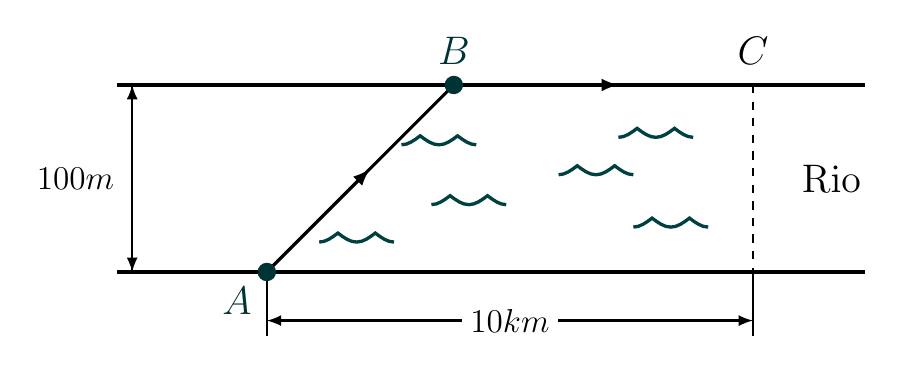
\begin{tikzpicture}[>=latex, scale=0.95]
    \coordinate (A) at (1.5, 0);
    \coordinate (B) at (4.0, 2.5);
    \coordinate (C) at (8.0, 2.5);
    \coordinate (C_proj) at (8.0, 0);

    \draw[line width=1.2pt] (-0.5, 0) -- (9.5, 0);
    \draw[line width=1.2pt] (-0.5, 2.5) -- (9.5, 2.5);

    \draw[thick, dashed] (C) -- (C_proj);

    \draw[line width=1.1pt] (A) -- (B);
    \draw[line width=1.1pt, ->] (A) -- (2.875, 1.375);

    \draw[line width=1.1pt] (B) -- (C);
    \draw[line width=1.1pt, ->] (B) -- (6.2, 2.5);

    \def\ondinha#1#2{
        \draw[line width=1.2pt, teal!50!black] 
            (#1, #2) cos ++(0.25, 0.12) sin ++(0.25, -0.12) cos ++(0.25, 0.12) sin ++(0.25, -0.12);
    }

    \ondinha{3.3}{1.7}
    \ondinha{2.2}{0.4}
    \ondinha{3.7}{0.9}
    \ondinha{6.2}{1.8}
    \ondinha{5.4}{1.3}
    \ondinha{6.4}{0.6}

    \draw[thick] (-0.3, 0) -- (-0.3, 2.5);
    \draw[thick, ->] (-0.3, 1.6) -- (-0.3, 2.5);
    \draw[thick, ->] (-0.3, 0.9) -- (-0.3, 0);
    \node[left=3pt] at (-0.3, 1.25) {\large $100\text{ m}$};

    \draw[thick] (A) -- ++(0, -0.85);
    \draw[thick] (C_proj) -- ++(0, -0.85);
    \draw[thick, <->] (1.5, -0.65) -- (8.0, -0.65) node[midway, fill=white, inner sep=3pt] {\large $10\text{ km}$};

    \fill[teal!40!black] (A) circle (3.5pt) node[below left=2pt] {\Large $A$};
    \fill[teal!40!black] (B) circle (3.5pt) node[above=4pt] {\Large $B$};
    \node[above=4pt] at (C) {\Large $C$};
    \node[right=6pt] at (8.3, 1.25) {\Large Rio};
\end{tikzpicture}
\end{center}
\end{exercicio}

\begin{exercicio}[13]
Qual o ponto $P$ da curva $y = x^2$ que se encontra mais próximo de $(3, 0)$? Seja $P = (a, b)$ tal ponto; mostre que a reta que passa por $(3, 0)$ e $(a, b)$ é normal à curva em $(a, b)$.
\end{exercicio}

\begin{exercicio}[14]
Encontre o ponto da curva $y = \dfrac{2}{x}$, $x > 0$, que está mais próximo da origem.
\end{exercicio}

\begin{exercicio}[15]
Duas partículas $P$ e $Q$ movem-se, respectivamente, sobre os eixos $0x$ e $0y$. A função de posição de $P$ é $x = \sqrt{t}$ e a de $Q$, $y = t^2 - \dfrac{3}{4}$, $t \ge 0$. Determine o instante em que a distância entre $P$ e $Q$ seja a menor possível.
\end{exercicio}

\begin{exercicio}[16]
Seja $g$ definida e positiva no intervalo $I$. Seja $p \in I$. Prove: $p$ será ponto de máximo (ou de mínimo) de $h(x) = \sqrt{g(x)}$ em $I$, se e somente se $p$ for ponto de máximo (ou de mínimo) de $g$ em $I$.
\end{exercicio}

\begin{exercicio}[17]
Um sólido será construído acoplando-se a um cilindro circular reto, de altura $h$ e raio $r$, uma semiesfera de raio $r$. Deseja-se que a área da superfície do sólido seja $5\pi$. Determine $r$ e $h$ para que o volume seja máximo.

\begin{center}
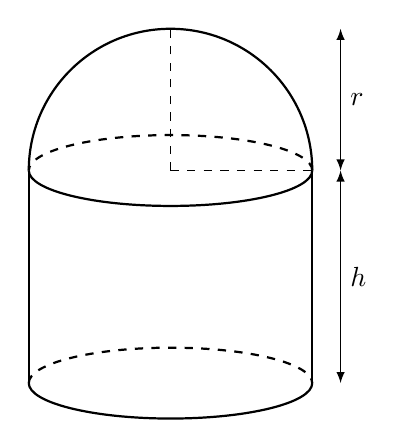
\begin{tikzpicture}[scale=0.9, >=latex]
    \draw[thick] (2, 3) arc (0:180:2);
    \draw[thick, dashed] (2, 3) arc (0:180:2 and 0.5);
    \draw[thick] (-2, 3) arc (-180:0:2 and 0.5);

    \draw[thick] (-2, 0) -- (-2, 3);
    \draw[thick] (2, 0) -- (2, 3);
    \draw[thick] (-2, 0) arc (-180:0:2 and 0.5);
    \draw[thick, dashed] (-2, 0) arc (180:0:2 and 0.5);

    \draw[dashed] (0, 3) -- (0, 5);
    \draw[dashed] (0, 3) -- (2, 3);
    \draw[<->] (2.4, 3) -- (2.4, 5) node[midway, right] {$r$};
    \draw[<->] (2.4, 0) -- (2.4, 3) node[midway, right] {$h$};
\end{tikzpicture}
\end{center}
\end{exercicio}

\begin{exercicio}[18]
A Cia. $\alpha$ Ltda. produz determinado produto e vende-o a um preço unitário de R\$ 13. Estima-se que o custo total $c$ para produzir e vender $q$ unidades é dado por $c = q^3 - 3q^2 + 4q + 2$. Supondo que toda a produção seja absorvida pelo mercado consumidor, que quantidade deverá ser produzida para se ter lucro máximo?
\end{exercicio}

\begin{exercicio}[19]
Determinado produto é produzido e vendido a um preço unitário $p$. O preço de venda não é constante, mas varia em função da quantidade $q$ demandada pelo mercado, de acordo com a equação $p = \sqrt{20 - q}$, $0 \le q \le 20$. Admita que, para produzir e vender uma unidade do produto, a empresa gasta em média R\$ 3,50. Que quantidade deverá ser produzida para que o lucro seja máximo?
\end{exercicio}

\begin{exercicio}[20]
Do ponto $A$, situado numa das margens de um rio, de $100\text{ m}$ de largura, deve-se levar energia elétrica ao ponto $C$ situado na outra margem do rio. O fio a ser utilizado na água custa R\$ 5 o metro, e o que será utilizado fora, R\$ 3 o metro. Como deverá ser feita a ligação para que o gasto com os fios seja o menor possível? (Suponha as margens retilíneas e paralelas.)

\begin{center}
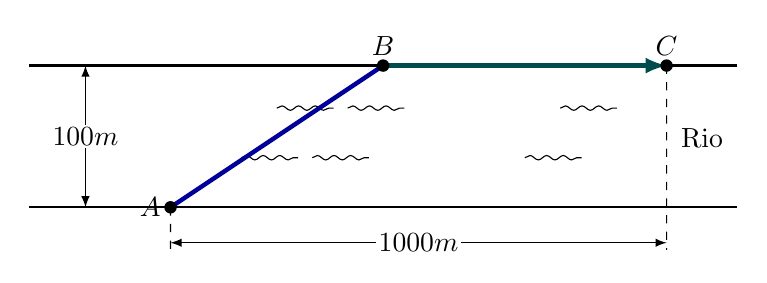
\begin{tikzpicture}[scale=0.9, >=latex]
    \draw[thick] (0, 0) -- (10, 0);
    \draw[thick] (0, 2) -- (10, 2);
    \node[above] at (9.5, 0.7) {Rio};

    \coordinate (A) at (2, 0);
    \coordinate (B) at (5, 2);
    \coordinate (C) at (9, 2);

    \foreach \x in {3, 4, 7} {
        \draw[decorate, decoration={snake, amplitude=0.8pt, segment length=6pt}] (\x, 0.7) -- ++(0.8, 0);
        \draw[decorate, decoration={snake, amplitude=0.8pt, segment length=6pt}] (\x+0.5, 1.4) -- ++(0.8, 0);
    }

    \draw[ultra thick, blue!60!black] (A) -- (B);
    \draw[ultra thick, ->, teal!60!black] (B) -- (C);

    \draw[dashed] (A) -- ++(-1.5, 0);
    \draw[dashed] (0, 2) -- ++(0.5, 0);
    \draw[<->] (0.8, 0) -- (0.8, 2) node[midway, fill=white, inner sep=1pt] {$100\text{ m}$};
    
    \draw[dashed] (A) -- (2, -0.6);
    \draw[dashed] (C) -- (9, -0.6);
    \draw[<->] (2, -0.5) -- (9, -0.5) node[midway, fill=white, inner sep=1pt] {$1000\text{ m}$};

    \fill (A) circle (2.5pt) node[left] {$A$};
    \fill (B) circle (2.5pt) node[above] {$B$};
    \fill (C) circle (2.5pt) node[above] {$C$};
\end{tikzpicture}
\end{center}
\end{exercicio}

\begin{exercicio}[21]
Sejam $P = (0, a)$ e $Q = (b, c)$, em que $a, b \text{ e } c$ são números reais dados e estritamente positivos. Seja $M = (x, 0)$, com $0 \le x \le b$.

\begin{center}
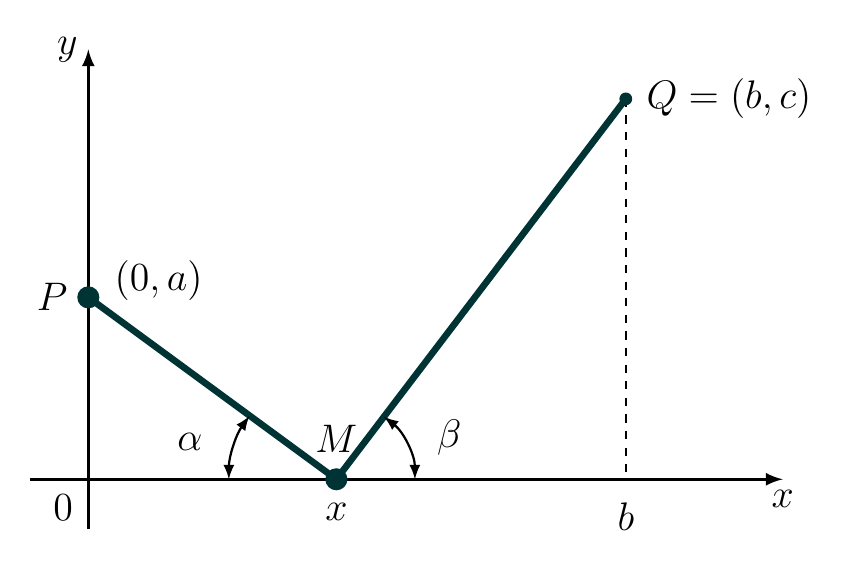
\begin{tikzpicture}[>=latex, scale=1.05]
    \coordinate (O) at (0, 0);
    \coordinate (P) at (0, 2.2);
    \coordinate (M) at (3.0, 0);
    \coordinate (Q) at (6.5, 4.6);
    \coordinate (Q_proj) at (6.5, 0);

    \draw[line width=1.1pt, ->] (-0.7, 0) -- (8.4, 0) node[below] {\Large $x$};
    \draw[line width=1.1pt, ->] (0, -0.6) -- (0, 5.2) node[left] {\Large $y$};
    \node[below left=2pt] at (O) {\Large $0$};

    \draw[thick, dashed] (Q) -- (Q_proj);

    \draw[line width=2.4pt, teal!40!black] (P) -- (M) -- (Q);

    \draw[thick, <->] (1.7, 0) arc (180:144:1.3);
    \node[left=3pt] at (1.6, 0.45) {\Large $\alpha$};

    \draw[thick, <->] (3.95, 0) arc (0:52.7:0.95);
    \node[right=3pt] at (4.0, 0.5) {\Large $\beta$};

    \fill[teal!40!black] (P) circle (3.8pt);
    \fill[teal!40!black] (M) circle (3.8pt);
    \fill[teal!40!black] (Q) circle (2.2pt);

    \node[left=4pt] at (P) {\Large $P$};
    \node[right=3pt] at (0.1, 2.4) {\Large $(0, a)$};
    \node[above=6pt] at (M) {\Large $M$};
    \node[below=5pt] at (M) {\Large $x$};
    \node[below=5pt] at (Q_proj) {\Large $b$};
    \node[right=4pt] at (Q) {\Large $Q = (b, c)$};
\end{tikzpicture}
\end{center}

\begin{enumerate}[label=\alph*)]
    \item Determine $x$ para que o perímetro do triângulo $PMQ$ seja mínimo.
    \item Conclua que o perímetro será mínimo para $\alpha = \beta$.
\end{enumerate}
\end{exercicio}

\begin{exercicio}[22]
Determine $M$ no gráfico de $y = x^3$, $0 \le x \le 1$, de modo que a área do triângulo de vértices $(0, 0)$, $(1, 1)$ e $M$ seja máxima.
\end{exercicio}

\begin{exercicio}[23]
A Cia. $\gamma$ Ltda. produz um determinado produto e vende-o com um lucro total dado por $L(q) = -q^3 + 12q^2 + 60q - 4$, em que $q$ representa a quantidade produzida. Determine o lucro máximo e a produção que maximiza o lucro. Esboce o gráfico desta função.
\end{exercicio}

\begin{exercicio}[24]
Determine uma reta tangente ao gráfico de $y = 1 - x^2$, de modo que a distância da origem a ela seja a menor possível.
\end{exercicio}

\begin{exercicio}[25]
Determine o ponto da parábola $y = 1 - x^2$ que se encontra mais próximo da origem.
\end{exercicio}

\begin{exercicio}[26]
Seja $(x_0, y_0)$, $x_0 > 0$ e $y_0 > 0$, um ponto da elipse $x^2 + 4y^2 = 1$. Seja $T$ a reta tangente à elipse no ponto $(x_0, y_0)$:
\begin{enumerate}[label=\alph*)]
    \item Verifique que $T$ tem por equação
    \[
    x_0 x + 4y_0 y = 1.
    \]
    \item Determine $x_0$ de modo que a área do triângulo determinado por $T$ e pelos eixos coordenados seja mínima.
\end{enumerate}
\end{exercicio}

\begin{exercicio}[27]
Uma partícula $P$ desloca-se sobre o eixo $x$ com velocidade constante e igual a 1. Outra partícula $Q$ desloca-se sobre a parábola $y = 1 - x^2$ de modo que sua projeção sobre o eixo $x$ descreve um movimento com velocidade constante e igual a 2. No instante $t = 0$, as partículas $P$ e $Q$ encontram-se, respectivamente, nas posições $(0, 0)$ e $(0, 1)$. Determine o instante em que as partículas encontram-se mais próximas.
\end{exercicio}

\begin{exercicio}[28]
Dado o triângulo retângulo de catetos 3 e 4, determine o retângulo de maior área nele inscrito, de modo que um dos lados esteja contido na hipotenusa.
\end{exercicio}

\begin{exercicio}[29]
Determine o ponto da parábola $y = x^2$ que se encontra mais próximo da reta $y = x - 2$.
\end{exercicio}

\begin{exercicio}[30]
Dois vértices de um retângulo $R$ estão sobre o eixo $x$ e os outros dois sobre o gráfico de $y = \dfrac{x}{1 + x^2}$, $x > 0$. Considere o cilindro que se obtém girando o retângulo $R$ em torno do eixo $x$. Determine o retângulo $R$ de modo que o volume do cilindro seja o maior possível.
\end{exercicio}

\begin{exercicio}[31]
Considere duas retas paralelas $r$ e $s$. Sejam $A$ e $C$ dois pontos distintos de $r$ e $B$ um ponto de $s$:

\begin{center}
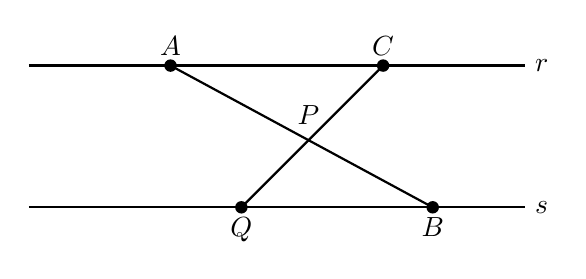
\begin{tikzpicture}[scale=0.9, >=latex]
    \draw[thick] (-1.5, 2) -- (5.5, 2) node[right] {$r$};
    \draw[thick] (-1.5, 0) -- (5.5, 0) node[right] {$s$};

    \coordinate (A) at (0.5, 2);
    \coordinate (C) at (3.5, 2);
    \coordinate (Q) at (1.5, 0);
    \coordinate (B) at (4.2, 0);

    \draw[thick] (A) -- (B);
    \draw[thick] (Q) -- (C);

    \coordinate (P) at (intersection of A--B and Q--C);

    \fill (A) circle (2.5pt) node[above] {$A$};
    \fill (C) circle (2.5pt) node[above] {$C$};
    \fill (Q) circle (2.5pt) node[below] {$Q$};
    \fill (B) circle (2.5pt) node[below] {$B$};
    \node[above=2pt] at (P) {$P$};
\end{tikzpicture}
\end{center}

Determine $Q$ na reta $s$ de modo que a soma das áreas dos triângulos $APC$ e $QPB$ seja mínima.
\end{exercicio}

\begin{exercicio}[32]
Considere o triângulo isósceles $ABC$, com $AB = BC$. Seja $H$ o ponto médio de $AC$. Determine $P$ no segmento $HB$ de modo que a soma das distâncias de $P$ aos pontos $A$, $B$ e $C$ seja a menor possível.
\end{exercicio}

\begin{exercicio}[33]
(\textbf{Lei de refração de Snellius.}) Considere uma reta $r$ e dois pontos $P$ e $Q$ localizados em semiplanos opostos:

\begin{center}
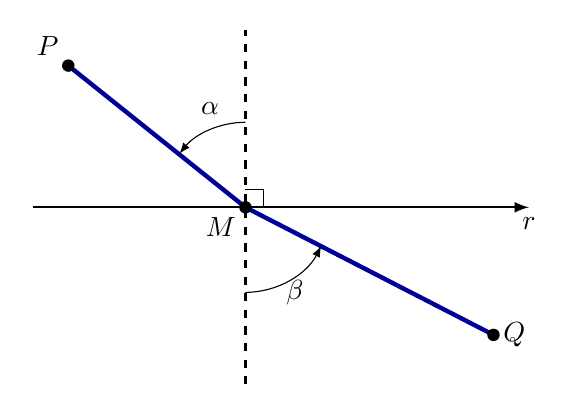
\begin{tikzpicture}[scale=0.9, >=latex]
    \draw[->, thick] (-1, 0) -- (6, 0) node[below] {$r$};
    \draw[dashed, thick] (2, -2.5) -- (2, 2.5);

    \coordinate (M) at (2, 0);
    \coordinate (P) at (-0.5, 2);
    \coordinate (Q) at (5.5, -1.8);

    \draw[ultra thick, blue!60!black] (P) -- (M);
    \draw[ultra thick, blue!60!black] (M) -- (Q);

    \draw (2, 0.25) -- (2.25, 0.25) -- (2.25, 0);

    \draw[->] (2, 1.2) arc (90:141:1.2);
    \node at (1.5, 1.4) {$\alpha$};

    \draw[->] (2, -1.2) arc (-90:-27:1.2);
    \node at (2.7, -1.2) {$\beta$};

    \fill (P) circle (2.5pt) node[above left] {$P$};
    \fill (M) circle (2.5pt) node[below left] {$M$};
    \fill (Q) circle (2.5pt) node[right] {$Q$};
\end{tikzpicture}
\end{center}

Uma partícula vai de $P$ a $M$ com velocidade constante $u$ e movimento retilíneo; em seguida, vai de $M$ a $Q$ com velocidade constante $v$, também com movimento retilíneo. Mostre que o tempo de percurso será mínimo se:
\[
\dfrac{\sen\alpha}{u} = \dfrac{\sen\beta}{v}.
\]
\end{exercicio}

\clearpage

% ==============================================================================
% 9.7. CONDIÇÃO NECESSÁRIA E CONDIÇÕES SUFICIENTES PARA MÁXIMOS E MÍNIMOS LOCAIS
% ==============================================================================
\subsection{Condição Necessária e Condições Suficientes para Máximos e Mínimos Locais}

\begin{exercicio}[1]
Determine os pontos críticos da função dada e classifique-os (a classificação refere-se a ponto de máximo local, ponto de mínimo local ou ponto de inflexão):
\begin{enumerate}[label=\alph*)]
    \item $f(x) = \dfrac{x^4}{4} - x^3 - 2x^2 + 3$
    \item $x(t) = \sqrt[3]{t^3 - 2t + 1}$
    \item $h(x) = x^3 - 3x^2 + 3x - 1$
    \item $f(x) = \dfrac{1}{x^4 + 2x^3 + x^2 + 1}$
    \item $f(x) = x^4 - 4x^3 + 6x^2 - 4x + 1$
    \item $g(x) = x^2 e^{-5x}$
\end{enumerate}
\end{exercicio}

\begin{exercicio}[2]
Suponha que $f$ admite derivada de 3\textsuperscript{a} ordem contínua no intervalo aberto $I$ e seja $p \in I$. Prove que se $f'(p) = f''(p) = 0$ e $f'''(p) \neq 0$, então $p$ é ponto de inflexão horizontal.
\end{exercicio}

\begin{exercicio}[3]
Suponha que $f$ admite derivada até a 4\textsuperscript{a} ordem contínua no intervalo aberto $I$ e seja $p \in I$. Prove que se $f'(p) = f''(p) = f'''(p) = 0$ e $f^{(4)}(p) \neq 0$, então $p$ será ponto de máximo local se $f^{(4)}(p) < 0$ e será ponto de mínimo local se $f^{(4)}(p) > 0$.
\end{exercicio}

\begin{exercicio}[4]
Generalize os resultados obtidos nos Exercícios 2 e 3.
\end{exercicio}

\begin{exercicio}[5]
Seja $f$ derivável em $\R$ e seja $g$ dada por $g(x) = \dfrac{f(x)}{x}$, $x \neq 0$. Suponha que $p$ é ponto de máximo local de $g$:
\begin{enumerate}[label=\alph*)]
    \item Prove que $pf'(p) - f(p) = 0$.
    \item Prove que a reta tangente ao gráfico de $f$ no ponto de abcissa $p$ passa pela origem.
\end{enumerate}
\end{exercicio}

\begin{exercicio}[6]
Suponha que $f$ seja derivável até a 2\textsuperscript{a} ordem em $\R$ e tal que para todo $x$:
\[
f''(x) + x\,f'(x) = 1.
\]
\begin{enumerate}[label=\alph*)]
    \item Prove que $f$ não admite ponto de máximo local.
    \item Prove que, se $f$ admitir um ponto crítico $x_0$, então $x_0$ será ponto de mínimo local.
    \item Prove que $f$ poderá admitir no máximo um ponto crítico.
\end{enumerate}
\end{exercicio}

\begin{exercicio}[7]
Suponha que $f$ seja derivável até a 2\textsuperscript{a} ordem em $\R$ e tal que para todo $x$:
\[
x\,f''(x) + f'(x) = 2.
\]
\begin{enumerate}[label=\alph*)]
    \item Prove que, se $x_0$ for ponto de máximo local, então $x_0 < 0$.
    \item Prove que, se $x_0$ for ponto de mínimo local, então $x_0 > 0$.
    \item Prove que $f'(x) > 0$ para todo $x$.\\
    (\textit{Sugestão:} Observe que $f'(0) = 2$.)
\end{enumerate}
\end{exercicio}

\begin{exercicio}[8]
(\textbf{Teorema de Darboux.}) Suponha $g$ derivável em $[a, b]$, com $g'(a) < 0$ e $g'(b) > 0$. Prove que existe $c \in {]a, b[}$ tal que $g'(c) = 0$. Interprete geometricamente.\\
(\textit{Sugestão:} Verifique que o valor mínimo $g(c)$ de $g$ em $[a, b]$ é tal que $g(c) < g(a)$ e $g(c) < g(b)$.)
\end{exercicio}

\begin{exercicio}[9]
Suponha $g$ derivável no intervalo $I$ e tal que $g'(x) \neq 0$ em todo $x$ de $I$. Prove que:
\[
g'(x) > 0 \text{ em todo } x \in I \quad\text{ou}\quad g'(x) < 0 \text{ em todo } x \in I.
\]
\end{exercicio}

\begin{exercicio}[10]
Suponha $g$ derivável em $[a, b]$ e seja $m$ tal que $g'(a) < m < g'(b)$. Prove que existe $c \in {]a, b[}$ tal que $g'(c) = m$.\\
(\textit{Sugestão:} Aplique o Exercício 8 à função $f(x) = g(x) - mx$.)
\end{exercicio}

\begin{exercicio}[11]
Seja $y = f(x)$ uma função derivável até a 2\textsuperscript{a} ordem no intervalo aberto $I$, tal que para todo $x \in I$:
\[
f''(x) + x\,f'(x) - [f(x)]^2 = 0 \quad\text{e}\quad f(x) \neq 0.
\]
\begin{enumerate}[label=\alph*)]
    \item Verifique que $f''$ é contínua em $I$.
    \item Prove que $f$ não admite ponto de máximo local em $I$.
\end{enumerate}
\end{exercicio}

\begin{exercicio}[12]
Seja $y = f(x)$ derivável até a 2\textsuperscript{a} ordem em ${]-r, r[}$, $r > 0$, tal que, para todo $x \in {]-r, r[}$:
\[
f''(x) + f'(x) - x[f(x)]^2 = 0.
\]
Suponha, ainda, que $f(0) = 0$ e $f'(0) = 1$.
\begin{enumerate}[label=\alph*)]
    \item Prove que $f$ não admite ponto de máximo local em ${]0, r[}$.
    \item Prove que $f$ não admite ponto de mínimo local em ${]-r, 0[}$.
    \item Prove que $f$ é estritamente crescente em ${]-r, r[}$.
\end{enumerate}
\end{exercicio}

\clearpage

% ==============================================================================
% 9.8. MÁXIMO E MÍNIMO DE FUNÇÃO CONTÍNUA EM INTERVALO FECHADO
% ==============================================================================
\subsection{Máximo e Mínimo de Função Contínua em Intervalo Fechado}

\begin{exercicio}[1]
Determine os valores máximos e mínimos (caso existam) de $f(x) = \dfrac{x^4}{4} - x^3 - 2x^2 + 3$ em $[-2, 3]$.
\end{exercicio}

\begin{exercicio}[2]
Determine os valores máximos e mínimos (caso existam) de $g(x) = x^3 - 3x^2 + 3x - 1$ em $[-2, 1]$.
\end{exercicio}

\begin{exercicio}[3]
Determine os valores máximos e mínimos (caso existam) de $f(x) = \dfrac{x^5}{5} - \dfrac{x^4}{2} - x^3 + 4x^2 - 4x + 1$ em $[-3, 3]$.
\end{exercicio}

\begin{exercicio}[4]
Determine os valores máximos e mínimos (caso existam) de $f(x) = \sen x - \cos x$ em $[0, \pi]$.
\end{exercicio}

\begin{exercicio}[5]
Determine os valores máximos e mínimos (caso existam) de $f(x) = \sqrt[3]{x^3 - 2x^2}$ em $[-1, 2]$.
\end{exercicio}

\begin{exercicio}[6]
Determine os valores máximos e mínimos (caso existam) de $f(x) = \dfrac{1}{x^3 - 2x^2}$ em ${]0, 2[}$.
\end{exercicio}
